\PassOptionsToPackage{table}{xcolor}
\documentclass[aspectratio=169]{beamer}\usepackage[utf8]{inputenc}
\usepackage{lmodern}
\usepackage[english]{babel}
\usepackage{color}
\usepackage{amsmath,mathtools}
\usepackage{booktabs}
\usepackage{mathptmx}
\usepackage[11pt]{moresize}
\usepackage{hyperref}
\usepackage{commath}
\usepackage{bm}
\usepackage{subfigure}
\usepackage{siunitx}

\setbeamertemplate{navigation symbols}{}
\setbeamersize{text margin left=5mm,text margin right=5mm}
\setbeamertemplate{caption}[numbered]
\addtobeamertemplate{navigation symbols}{}{
\usebeamerfont{footline}
\usebeamercolor[fg]{footline}
\hspace{1em}
\insertframenumber/\inserttotalframenumber}

\newcommand{\R}{\mathbb{R}}
\newcommand{\E}{\mathbb{E}}
\newcommand{\N}{\mathbb{N}}
\newcommand{\Z}{\mathbb{Z}}
\newcommand{\V}{\mathbb{V}}
\newcommand{\Q}{\mathbb{Q}}
\newcommand{\K}{\mathbb{K}}
\newcommand{\C}{\mathbb{C}}
\newcommand{\T}{\mathbb{T}}
\newcommand{\I}{\mathbb{I}}

\title{Cross Correlation Function}
\subtitle{Renzo Miguel Caballero Rosas}

\begin{document}

\begin{frame}
\titlepage
\end{frame}

%%%%%%%%%%%%%%%%%%%%%%%%%%%%%%%%%%%

\setbeamercolor{background canvas}{bg=white!10}
\begin{frame}\frametitle{Cross-correlation Function for the error observations $\{v_{j,i}\}_{j=1,i=1}^{M,N}$:}

\begin{figure}[ht!]
\centering
\includegraphics[width=0.6\textwidth]{obs_alldata.eps}
\end{figure}

\end{frame}

%%%%%%%%%%%%%%%%%%%%%%%%%%%%%%%%%%%

\setbeamercolor{background canvas}{bg=white!10}
\begin{frame}\frametitle{Cross-correlation Function for the error observations $\{v_{j,i}\}_{j=1,i=1}^{M,N}$:}

\begin{figure}[ht!]
\centering
\includegraphics[width=0.6\textwidth]{obs_training.eps}
\end{figure}

\end{frame}

%%%%%%%%%%%%%%%%%%%%%%%%%%%%%%%%%%%

\setbeamercolor{background canvas}{bg=white!10}
\begin{frame}\frametitle{Cross-correlation Function for the transitions $\{\Delta v_{j,i}\}_{j=1,i=1}^{M,N}$:}

\begin{figure}[ht!]
\centering
\includegraphics[width=0.6\textwidth]{tran_alldata.eps}
\end{figure}

\end{frame}

%%%%%%%%%%%%%%%%%%%%%%%%%%%%%%%%%%%

\setbeamercolor{background canvas}{bg=white!10}
\begin{frame}\frametitle{Cross-correlation Function for the transitions $\{\Delta v_{j,i}\}_{j=1,i=1}^{M,N}$:}

\begin{figure}[ht!]
\centering
\includegraphics[width=0.6\textwidth]{tran_training.eps}
\end{figure}

\end{frame}

%%%%%%%%%%%%%%%%%%%%%%%%%%%%%%%%%%%

\end{document}